Tunnistautumisessa on kolme osapuolta: asiakasohjelma, web-palvelu ja tunnistautumispalvelu \cite{nisti}. Osapuolet on esitetty kuvassa \ref{composition}, jossa on mukana myös tunnistautumispalvelun käyttämä käyttäjähallinta. Käyttäjähallinta voi olla osa tunnistautumispalvelua tai oma komponenttinsa. Tunnistautumisen kannalta sillä, onko käyttäjähallinta osa tunnistautumispalvelu vai erillinen komponentti, ei ole merkitystä.

\begin{figure}[ht]
\centering
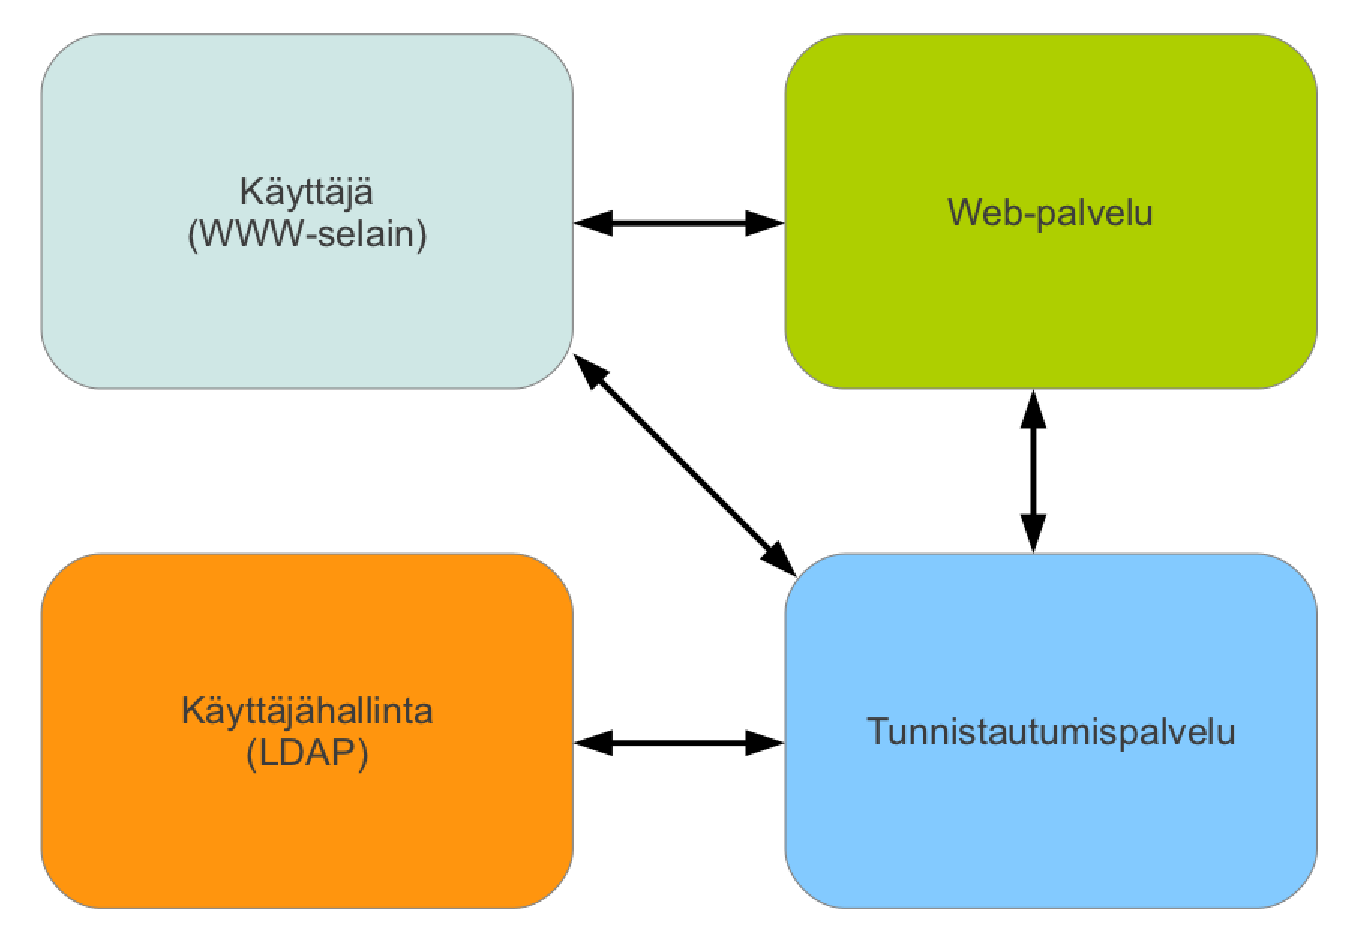
\includegraphics[width=0.7\textwidth]{teknologiat/composition.eps}
\caption{Keskitetyn tunnistautumisen osapuolet.}%
\label{composition}
\end{figure}

Ensimmäiseksi käyttäjä menee asiakasohjelmalla web-palveluun, joka pyytää tunnistautumista erillisessä tunnistautumispalvelussa. Käyttäjän asiakasohjelma ohjataan tunnistautumispalvelun sivulle, joka on yhteydessä organisaation käyttäjähallintaan. Sen mukaan mitä rajapintaprotokollaa käytetään, käyttäjälle joko palautetaan todistus siitä, että hän on se, joka väittää olevansa, tai avain, jonka avulla web-palvelu voi hakea käyttäjän tiedot tunnistautumispalvelulta. Tunnistautumisprotokollia (kuten SAML, OpenID) käytettäessä käyttäjälle palautetaan tunnistautumispalvelun allekirjoittama valtuutustieto, joka vahvistaa käyttäjän identiteetin \cite{nisti}.

Pääsynhallintaprotokollien (esim. OAuth) kohdalla käytetään ns. näennäistunnistautumista (pseudo authentication), jolloin web-palvelu hakee valtuutusavaimella käyttäjän tiedot tunnistautumispalvelusta \cite{distributed_web_security}. Käyttäjän identiteettiä ei siis suoraan varmenneta, mutta koska käyttäjällä on hallussaan avain, jolla pääsee tietoihinsa käsiksi, oletetaan käyttäjän olevan se, jonka tiedot avaimeen liittyvät.

Useimmat tunnistautumisen vaiheet tapahtuvat käyttäjältä näkymättömissä selaimen uudelleenohjauksen yhteydessä. Käyttäjälle näkyvä vaihe on kirjautuminen tunnistautumispalveluun, jolloin häneltä pyydetään käyttäjätunnus sekä salasana. Käyttäjän syötettä vaativat vaiheet on esitetty aiemmassa kuvassa \ref{facebook_login}.